%% ------------------------------------------------------------------------- %%
\chapter{Decomposição em Baldes}
\label{cap:decomp-raiz}

\section{Introdução}

Na seção anterior desenvolvemos um algoritmo simples que percorre, no pior caso, todos os vértices de uma árvore. Neste capítulo apresentaremos uma otimização ao algoritmo anterior para que sua complexidade de tempo seja $O(\sqrt{n})$.

\section{Otimização}

A ideia do algoritmo que vamos desenvolver é a mesma descrita no Algoritmo 3. Isto é, para dois vértices $a$ e $b$ ainda vamos percorrer seus caminhos até a raiz para determinar o seu \LCA.

A diferença é que agora não vamos potencialmente visitar todos os vértices do caminho até encontrar o \LCA. Agora, vamos dividir os vértices da árvore em "baldes", para que inicialmente um pulo entre dois membros do caminho seja de um vértice de um balde para um vértice de outro balde, ao invés de ir para o seu pai direto. Assim, um pulo não tem mais tamanho 1, mas sim $b$, onde $b$ é a altura de um balde.

\subsection{Detalhando o algoritmo}

Assumindo que as profundidades dos vértices já foram calculadas, vamos criar alguns baldes de forma que:

\begin{itemize}
    \item O balde número 1 tenha todos os vértices de profundidade [$1$...$p$];
    \item O balde número 2 tenha todos os vértices de profundidade [$p+1$...$2p$];
    \item O balde número 3 tenha todos os vértices de profundidade [$2p+1$...$3p$];
    \item etc.
\end{itemize}

O valor de $p$ é essencial para que a otimização do algoritmo seja feita. Entraremos em mais detalhes em como obtê-lo na seção ~\ref{complexidade-balde}, onde analisaremos a complexidade do código que desenvolveremos.

Em nosso algoritmo precisamos guardar, para cada vértice de um balde, quem é o seu ancestral mais profundo do balde anterior. Para melhor ilustrar isso, apresentamos a figura~\ref{fig:arvore-baldes}:

\begin{figure}[htb]
\begin{center}
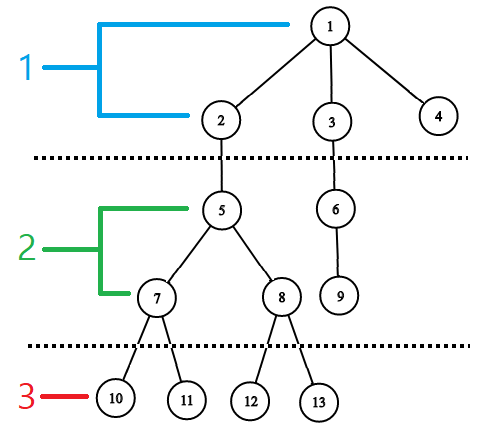
\includegraphics[width=11cm]{images/tree_buckets.png}
\end{center}
\caption{\label{fig:arvore-baldes}Divisão dos vértices em baldes (1, 2 e 3).}
\end{figure}

Neste exemplo temos 5 níveis de profundidades e escolhemos o valor de $p = 2$. Entretanto, como 5 não é divisível por 2, temos que os dois primeiros baldes possuam de fato $p = 2$ níveis de profundidade enquanto o terceiro tem o restante (ou seja, 1).

A partir desta árvore podemos construir tais ancestrais mais profundos do balde anterior do seguinte modo:

\begin{table}[htb]
\centering
\begin{tabular}{|l|c|c|c|c|c|c|c|c|c|c|c|c|c|c|}
\hline
Vértice   & 1 & 2 & 3 & 4 & 5 & 6 & 7 & 8 & 9 & 10 & 11 & 12 & 13 \\ \hline
Ancestral & 1 & 1 & 1 & 1 & 2 & 3 & 2 & 2 & 3 & 7  & 7  & 8  & 8 \\ \hline
\end{tabular}
\caption{Ancestrais mais profundos do balde anterior para cada vértice}
\end{table}

Note que o ancestral da raiz é naturalmente ela mesma.

Então, para encontrar o \LCA\ entre dois vértices $a$ e $b$ basta verificar em qual balde o \LCA\ está (isto é, percorrer os caminhos de $a$ e $b$ para a raiz até que os ancestrais do balde anterior sejam iguais), e daí trivialmente encontrá-lo.

Por exemplo, se quisermos encontrar o \LCA\ entre os vértices \textbf{10} e \textbf{13}, faríamos o seguinte:

\begin{itemize}
    \item Ancestral de 10 é o vértice \textbf{7}. Ancestral de 13 é o vértice \textbf{8}. Como são vértices distintos, atualizamos nossos vértices para seus ancestrais.
    \item Ancestral de 7 é o vértice \textbf{2}. Ancestral de 8 é o vértice \textbf{2}. Como seus ancestrais do balde anterior são o mesmo vértice, sabemos que o \LCA\ está no balde atual (ou então é o próprio vértice 2, que já é comum aos dois).
\end{itemize}
Agora, basta percorrer os caminhos de \textbf{7} e \textbf{8} até a raiz naturalmente, dando pulos de tamanho 1 (isto é, indo aos seus pais diretos).
\begin{itemize}
    \item Pai de 7 é o vértice \textbf{5}. Pai de 8 é o vértice \textbf{5}. Como seus pais são iguais, podemos afirmar que este é o \LCA\ do nosso problema.
\end{itemize}

\section{Código}

Utilizaremos os algoritmos 2 e 3 demonstrados anteriormente. Veremos que precisamos de poucas adições neles para que fiquem otimizados.

Como dito anteriormente, além da profundidade, também guardaremos para cada vértice quem é o seu ancestral mais profundo do balde anterior utilizando os vetores globais $profundidade$ e $baldeAnterior$, respectivamente. Além disso, toda vez que o nível atual for múltiplo da altura do balde permitido ($p$ citado anteriormente)  "criaremos"\ um novo balde.

\vspace{0.3cm}

\begin{algorithm}[H]
\caption{Modificação do algoritmo 2}
\begin{algorithmic}[1]
\Function{\textsc{CalculaProfundidade}}{vertice,\ nivel,\ ancestralAnterior}
    \State $profundidade[vertice] \rec nivel$
    \State $baldeAnterior[vertice] \rec ancestralAnterior$
    \If{$nivel \ \% \ alturaBalde = 0$}
        \State $anterior \rec vertice$
    \Else
        \State $anterior \rec ancestralAnterior$
    \EndIf
    \For{cada $filho$ em $filhos[vertice]$}
        \State $CalculaProfundidade(filho,\ nivel+1,\ anterior)$
    \EndFor
\EndFunction
\end{algorithmic}
\end{algorithm}

Para a função que determina o \LCA, primeiro faremos com que $a$ e $b$ estejam no mesmo balde cujo ancestral anterior seja o mesmo para ambos. Após isso, basta chamar a função de \LCA\ simples, demonstrada no algoritmo 3.

\vspace{0.3cm}

\begin{algorithm}[H]
\caption{\LCA\ utilizando o conceito de baldes}
\begin{algorithmic}[1]
\Function{\textsc{LCA}}{a,\ b}
    \While { $baldeAnterior[a]$ != $baldeAnterior[b]$}
        \If{$profundidade[a] < profundidade[b]$}
            \State $troca(a,\ b)$
        \State $a \rec baldeAnterior[a]$
        \EndIf
    \EndWhile
    \\\hspace{5mm} \Return $LCA\_Simples(a,\ b)$
\EndFunction
\end{algorithmic}
\end{algorithm}

\subsection{Corretude}

Assumindo o algoritmo 4 como correto, a ideia do algoritmo 5 é similar à apresentada no algoritmo 3: após a execução do laço da linha 2 teremos dois vértices no mesmo balde cujos ancestrais do balde anterior são os mesmos. Afinal, sabemos que percorrer o caminho de um vértice pulando de balde em balde resultará no mesmo destino do algoritmo 3, que caminha vértice após vértice: a raiz. Isso se deve ao fato de que no algoritmo 4 apresentado nessa seção, o objeto $baldeAnterior$ apenas serve como um encurtador de caminhos - mais precisamente deixando cada pulo em um caminho de  tamanho $alturaBalde$ (isto é, a partir de um vértice de profundidade $p$ chegamos em outro de profundidade $p - alturaBalde$).

A linha 5 do código atualiza o valor de $a$ para o próximo vértice do seu caminho encurtado até a raiz. Sabemos que $a$ sempre é mais profundo do que $b$ já que as linhas 3 e 4 trocam os vértices $a$ e $b$ caso o segundo seja mais profundo do que o primeiro.

O código termina com uma chamada da função LCA\_Simples já provada no capítulo anterior, que devolve o \LCA\ entre dois vértices de uma árvore enraizada.

\subsection{Complexidade}
\label{complexidade-balde}

O algoritmo 4 executa uma simples busca em profundidade com operações de tempo constante (linhas 2-7) e assim sua complexidade de tempo é $O(n+m)$, onde $n$ é a quantidade de vértices e $m$ a quantidade de arestas. A complexidade de espaço é $O(n)$.

Seja $q$ a quantidade de baldes existentes. No laço das linhas 2-5 do algoritmo 5, sendo $q_a$ e $q_b$ as quantidades de baldes acima de $a$ e $b$, respectivamente, em seus caminhos até a raiz, podemos dizer que são executadas $q_a + q_b$ operações. No pior caso, $q_a = q_b = q$, e portanto essa etapa do algoritmo é $O(q)$.

A chamada de LCA\_Simples tem complexidade $O(h)$, onde $h$ é a altura da árvore (no pior caso a quantidade de vértices $n = h$, então é correto assumir tal complexidade). Entretanto, ao dividir nossa árvore em baldes, garantimos que qualquer balde terá altura $h = alturaBalde$.

Assim, denotando $p = alturaBalde$, o algoritmo 5 tem complexidade de tempo $O(p + q)$. Dado que os valores $p$ e $q$ dependem diretamente da condição de inserção de um vértice em um balde, analisemos agora como fazer isso para atingir a melhor complexidade possível.

\vspace{0.8cm}

\subsubsection{Tamanho de um balde}

Para que o algoritmo descrito fique de fato mais eficiente do que o do capítulo anterior, devemos escolher bem quantos níveis de profundidade vamos permitir que estejam em um mesmo balde. Ou seja, determinar, para cada balde, o tamanho do intervalo de profundidades que descrevemos anteriormente.

Queremos minimizar a soma $p + q$, (duas fases do algoritmo: avaliar $q$ baldes e percorrer $p$ vértices). Além disso, também vale que $pq = h$, onde $h$ é a altura da árvore. Então, nosso problema resume-se a:

\centerline{minimizar $p + q$}
\centerline{dado que $pq \leq h$}

\hspace{1cm}

Já que $p \geq 0$ e $q \geq 0$, temos que $(\sqrt{p} - \sqrt{q}))^2 \geq 0$

$\implies p + q \geq 2\sqrt{pq}$
$\implies p + q \geq 2\sqrt{h}$

\hspace{1cm}

Como o objetivo é minimizar $p + q$, queremos que $p + q = 2\sqrt{h}$. Para que isso aconteça, por sua vez, segue que $(\sqrt{p} - \sqrt{q}))^2 = 0 \implies p = q = \sqrt{h}$.

\hspace{1cm}

Vale notar que no pior caso a altura $h$ de uma árvore é igual à quantidade $n$ de vértices que ela possui. Portanto, concluímos que o tamanho ótimo de um balde é sempre $\sqrt{n}$ (com $\sqrt{n}$ baldes), e assim a complexidade de tempo do algoritmo é de fato $O(\sqrt{n})$.

